\documentclass[letterpaper,12pt,onecolumn]{article}

%10pt, 12pt,11pt
%PREAMBLE

%\usepackage{fullpage}%geometry


\usepackage{blindtext,setspace,soul}
\usepackage{multicol,xcolor,graphicx}

\usepackage{amsmath}

\begin{document}
\section{Table}

\begin{table}[t]
%\begin{center}
\centering
\caption{table name\label{tab:1}}
\end{table}
\section{figures}

\blindtext
%
\begin{figure}[ht]
%\begin{center}
\centering
%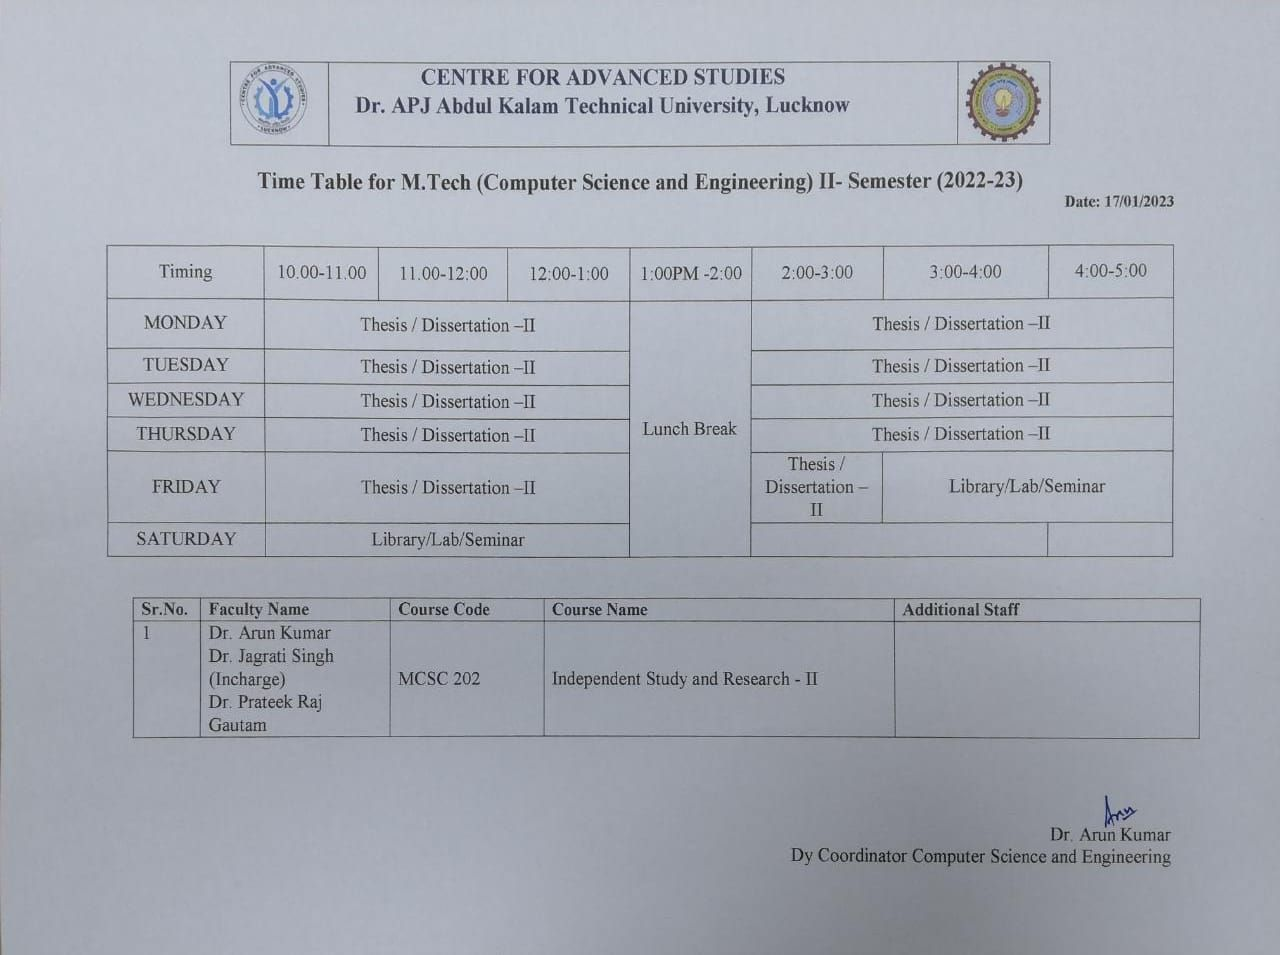
\includegraphics[width=.8\linewidth]{2.jpg}
\caption{Figure name\label{fig:1}}
%\end{center}
\end{figure}
\blindtext
\begin{figure}
%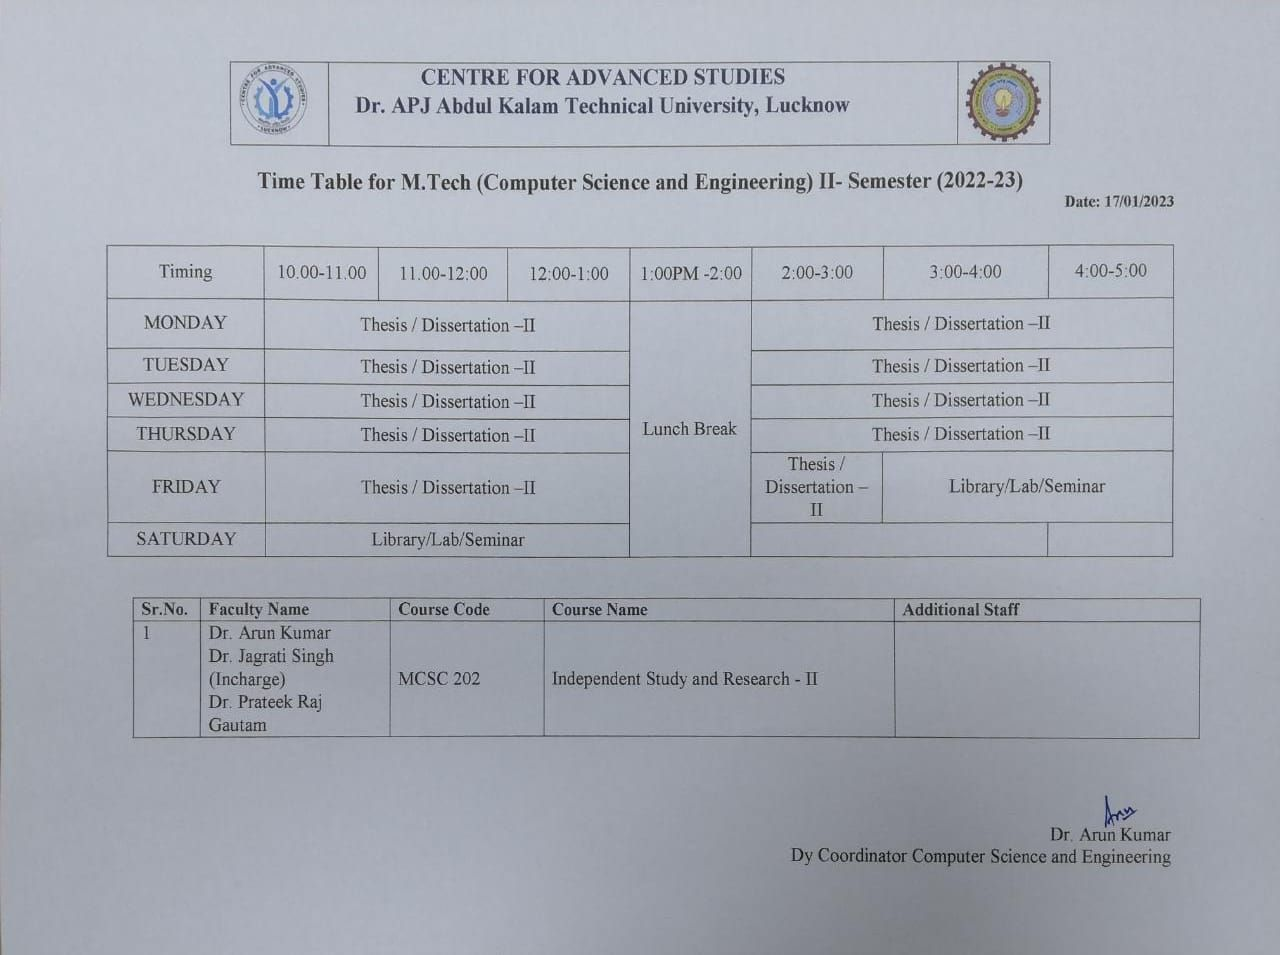
\includegraphics[width=.8\linewidth]{2.jpg}
\caption{Figure name\label{fig:1}}
\end{figure}
\blindtext
\blindtext
\begin{figure}
\begin{center}
%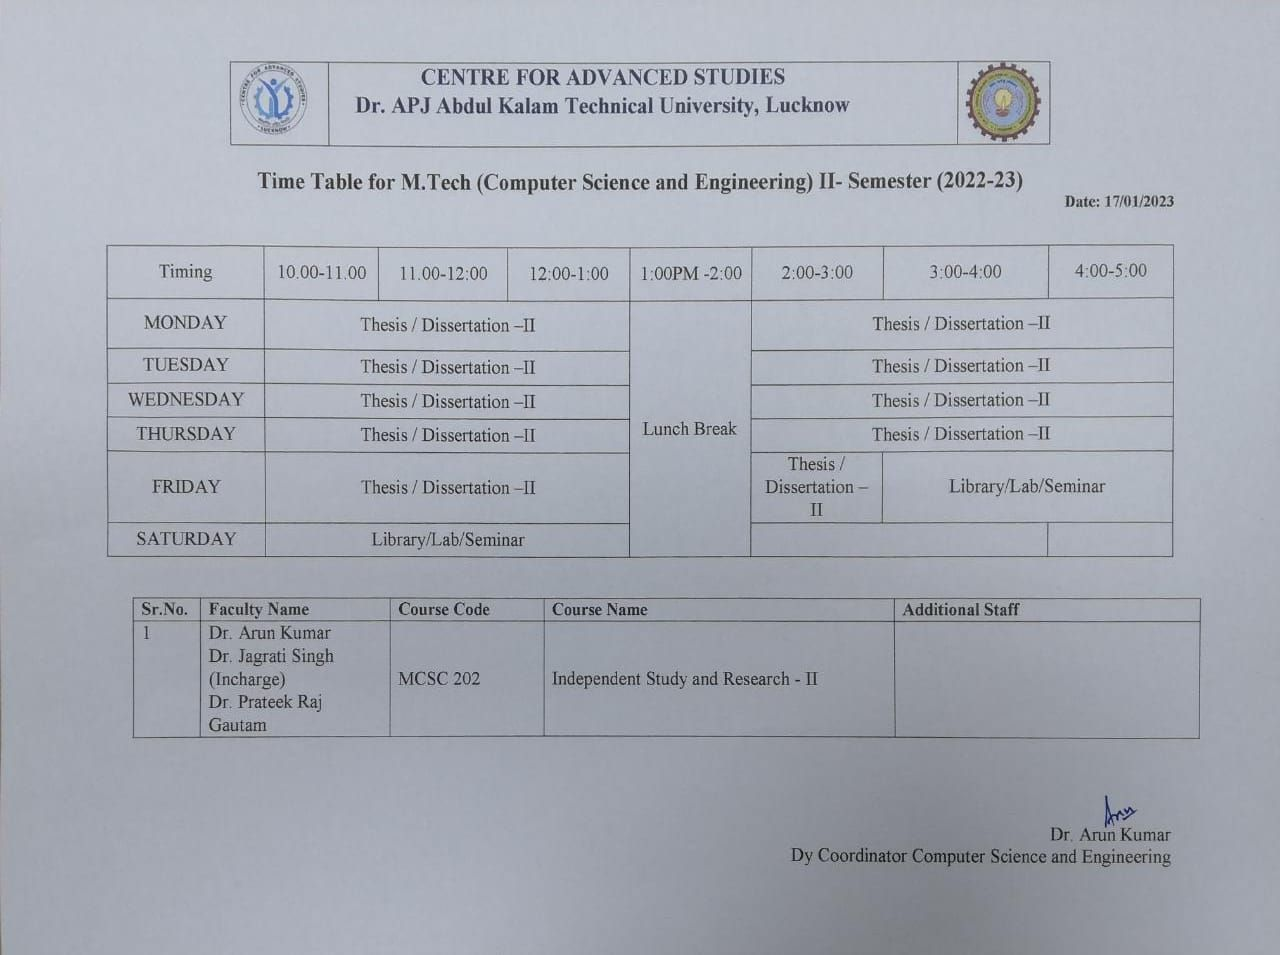
\includegraphics[width=.8\linewidth]{2.jpg}
\caption{Figure name\label{fig:1}}
\end{center}
\end{figure}
\blindtext
%{\tiny{tiny}}

{
\small{Small}
\footnotesize{fn}
\large{large}
\Large{Large}
\LARGE{LARGE}}
{\huge{huge}
}
\section{equations}
\color{red!40!black!10!blue}{\blindtext}
\so{adsfasdfavs asdfas\emph{emphasdfasdf} a sfvasdf}\\
\ul{adsfasdfavs asdfas\emph{emphasdfasdf} a sfvasdf}\\
\st{adsfasdfavs asdfas\emph{emphasdfasdf} a sfvasdf}\\
\caps{adsfasdfavs asdfas\emph{emphasdfasdf} a sfvasdf}\\
\hl{adsfasdfavs asdfas\emph{emphasdfasdf} a sfvasdf}\\
%i am defining eqn \eqref{eq:1}

%\begin{equation}
\begin{eqnarray}
A&=&\frac{B}{c}      \nonumber\\
&=&\frac{B_{New}}{c}\label{eqn:11}\\
A&=&\frac{B}{c}\nonumber\\
&=&\frac{B_{New}}{c}\label{eqn:12}
\end{eqnarray}

\begin{equation}
A+v\int_{0}^{\Omega} \sum_{i=0}^{\Omega}=\frac{B}{c}
\label{eq:2}
\end{equation}

\[
\]

\begin{equation}
\left\lfloor
\frac{a}{
\left(\frac{R}{X}^{code_b^x} \mathbf{R} 
\right)}
\right]\rfloor^{power}
\label{eq:2}
\end{equation}


\begin{equation}
\left\{\frac{a}{eqn}\right.
\label{eq:2}
\end{equation}


\begin{equation}
\left.\frac{a}{eqn}\right]
\label{eq:2}
\end{equation}


\doublespacing
\textbf{\blindtext}
\textit{\blindtext}
$E=mc^2$ $\eta$ $\int$ ${\sqrt\delta\Delta}$
$$\frac{num}{den}$$
\singlespacing
\onehalfspacing
\begin{equation}
F=ma
\label{eq:force}
\end{equation}



\begin{equation}
\overrightarrow{F}=m\vec{a}
\label{eq:force}
\end{equation}


\begin{equation}
F=ma\hat{a}
\label{eq:force}
\end{equation}
\blindtext equation \ref{eq:force}
%MAIN SECTION or DOCUMENT CONTENT

%\chapter{some new chapter}
%\part{A}
%\chapter{main chapter}

\label{fig:name}
{tab:name}






\begin{multicols}{3}

%first section
\section{Introduction}\label{sec:intro}
hello latex
hi \LaTeX
this is some random        
\subsection{subsection}     
\blindtext 
\subsubsection{subsection}    \blindtext  
\paragraph{paragraph heading} \blindtext
\subsection{subsection}        text 
\label{introTwo}
this is some random textadflksjdf;laksjdf
this is some random textasdfasdgasdgsdagasdgag asldgoijasdg
\end{multicols}











% second part

%
% \part{B}
%\chapter{ 2 main chapter}

\section{Introduction}
hello latex

\ref{intro} Refering here\\

\ref{introTwo} refer intro two\\
hi \LaTeX
this is some random        
\subsection{subsection}     
\blindtext 
\subsubsection{subsection}    \blindtext  
\paragraph{paragraph heading} \blindtext
\subsection{subsection}        text 

this is some random textadflksjdf;laksjdf
this is some random textasdfasdgasdgsdagasdgag asldgoijasdg aldsfgokapdofgpadofitextasdfasdg
asdgsdagasdgag asldgoijasdg aldsfgokapdofgpadofitextasdfasdg
asdgsdagasdgag asldgoijasdg aldsfgokapdofgpadofi
\par PARAGRAPH his is some random text
this is some random text
this is some random text

\section{METHOD}
this is some random text
this is some random text
this is some random text

\section{RESULTS}
\par PARAGRAPH his is some random text
this is some random text
this is some random text
this is some random text
this is some random text
this is some random text
\par\noindent NOINDENT PARAGRAPH his is some random text
this is some random text
this is some random text.\\NEWLINE this is some random text
this is some random text
this is some random text
\par PARAGRAPH his is \newline NEWLINE some random text
this is some random text
this is some random text
this is some random text
this is some random text
this is some random text
this is some random text
this is some random textt
this is some random text
this is some random text
this is some random text
this is some random text
this is some random text
this is some random text
this is some random text
this is some random text
this is some random text
this is some random text
this is some random textt
this is some random text
this is some random text
this is some random text
this is some random text
this is some random text
this is some random text
this is some random text
this is some random text
this is some random text
this is some random text
this is some random textt
this is some random text
this is some random text
this is some random text
this is some random text
this is some random text
this is some random text
this is some random text
this is some random text
this is some random text
this is some random text
this is some random textt
this is some random text
this is some random text
this is some random text
this is some random text
this is some random text
this is some random text
this is some random text
this is some random text
this is some random text
this is some random text
this is some random textt



\end{document}